\section{Stromrichter}
Die Leistungselektronik wir in einem mobilen Container, der für die Außenaufstellung ausgelegt wird untergebracht und verbindet die beiden Transformatoren.
Die Zwischenkreiskomponenten wie die Drosseln, Kondensatoren und Widerstände werden ebenfalls außen aufgestellt und mit dem COntainer verbuden. 

\subsection{Allgemeine Merkmale}
\begin{table}[htb]
    \centering
    \begin{NiceTabular}{|l|c|}[]
        \CodeBefore
        \columncolor{lightergray}{1}
        \Body
        \hline
         Aufstellung & Container(Innenraum)\\
         \hline
         Verschmutzung & Verschmutzungsgrad II (normal) \\
         \hline
         Aufstellungshöhe & < 1000 m üNN\\
         \hline
         Umgebungstemperatur &  -30°C bis 40°C\\
         \hline
         Klimabedingungen & Normal\\ 
         \hline
                 \Block{3-1}{Dokumentationen} &  \tabitem Technische Zeichnungen und CAD\\
                         &\tabitem Montageplan, Wartungsplan, Dokumentationen\\
                         &\tabitem Prüfprotokoll der zu erfüllenden Prüfungen\\
            \hline
    \end{NiceTabular}
\end{table}
\subsubsection*{Schaltbild}

\begin{figure}[!tbp]
    \centering
    \begin{minipage}[b]{0.5\textwidth}
        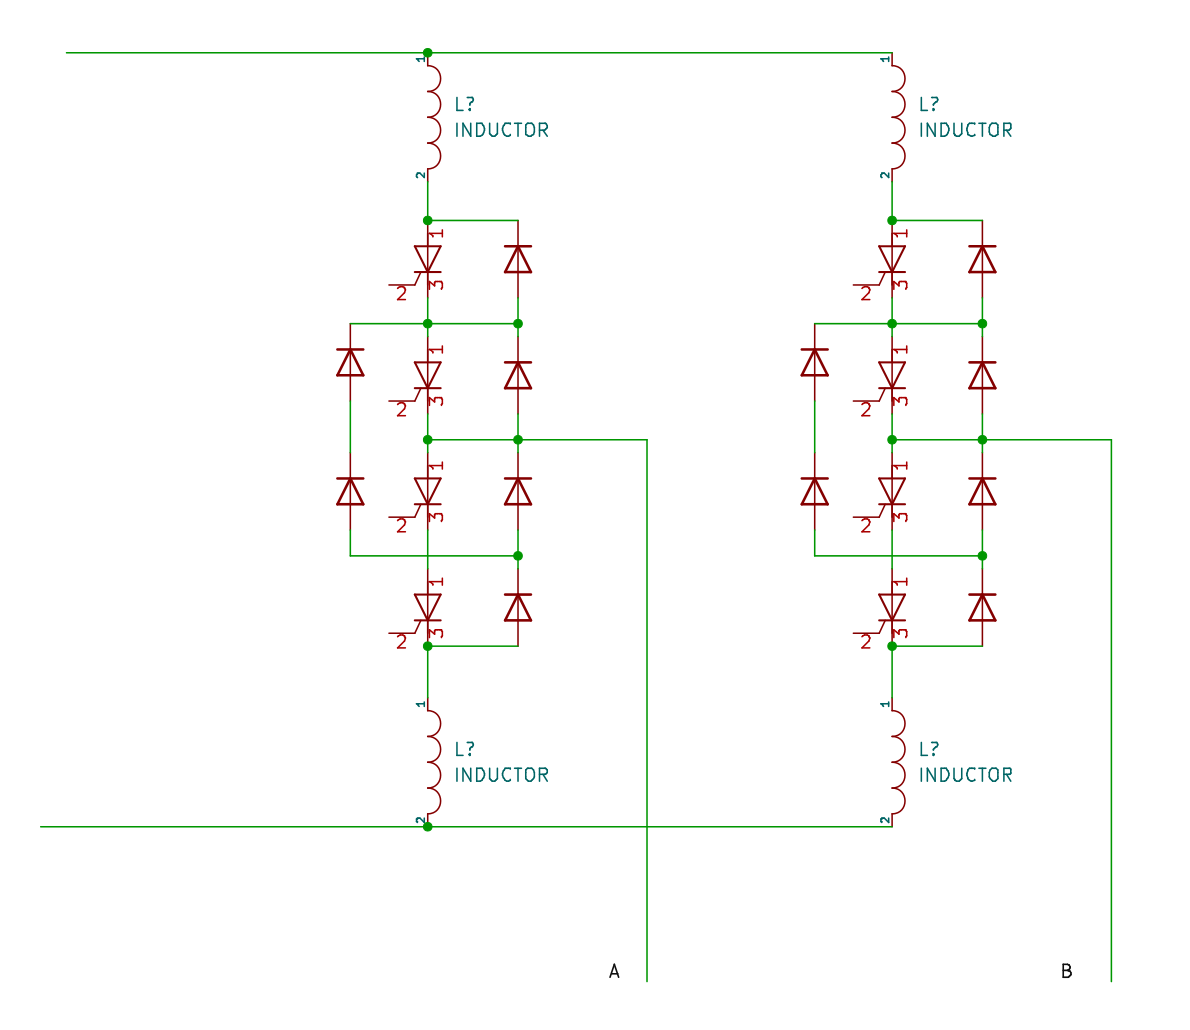
\includegraphics[width=\textwidth,frame]{Bilder/umrichter_schaltbild.png}
      \caption{3-Level 4QS}
    \end{minipage}
    \hfill
    \begin{minipage}[b]{0.4\textwidth}
        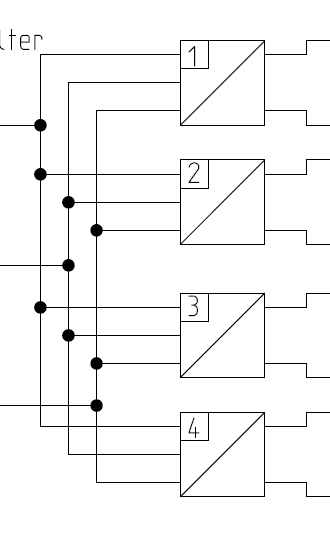
\includegraphics[width=\textwidth,frame]{Bilder/umrichter_16.png}
      \caption{Anschluss der Umrichter an Zwischenkreis und Summiertrafo}
    \end{minipage}
  \end{figure}


\subsection{Bemessungsdaten Umrichter}
\begin{table}[htb]
    \centering
    \begin{NiceTabular}{|l|p{4cm}|}[hvlines]
        \CodeBefore
        \columncolor{lightergray}{1}
        \Body
         Nennscheinleistung pro Umrichter& $\SI{5}{\unit{\mega\volt\ampere}}$\\
         Nennschwirkleistung pro Umrichter& $\SI{4}{\unit{\mega\watt}}$\\
         Nenneingangsspannung DC  & $\SI{5000}{\V}$\\
         Nennausgangaspannung AC (RMS) & $\SI{3535}{\V}$\\
         Nennfrequenz AC-Seite  & $\SI{16.7}{\Hz}-6\%+4\%$\cite*{DeutschesInstitutfurNormungene.V..200802}\\
         Wirkungsgrad& $>95\%$\\  
         Nennstrom DC pro Umrichter & $\SI[]{1}[]{\kilo\ampere}$  \\
         max. Strombelastung Halbleiter & \SI[]{1714}[]{\A}\\ 
         max. Spannungsbelastung Halbleiter & \SI[]{2500}[]{\V}\\
    \end{NiceTabular}
\end{table}


\subsubsection*{Kühlung}
Die Wechselrichter werden über ein autake Wasserkühlung gekühhlt. Pumpen befördern das Kühlwasser von den Halbleitern 
zum Wärmetauscher. Über diesen Wärmetauscher werden die Verluste des Wechselrichters an die Umgebung abgegeben. 

\subsection{Funktionsprüfung}

\begin{itemize}
    \item Spannungsprüfungen nach Isolationskoordinaten 
    \item Dummes scheiße
\end{itemize}

\subsubsection*{Normen}
\begin{itemize}
    \item DIN EN 60146-2: Halbleiter-Stromrichter Teil 2: Selbstgeführte Halbleiter-Stromrichter
    einschließlich Gleichstrom-Direktumrichter
\end{itemize}
                                                           